%%%%%%%%%%%%% Appendices %%%%%%%%%%%%%


\chapter{Appendix}
All the relevant files and progress data is available in \href{https://github.com/dakshinatharindu/Digital-Alarm-Clock}{this} Github repository.
\section{The PCB}
Schematics, PCB and table of content.
Used Altium Designer to design these models
%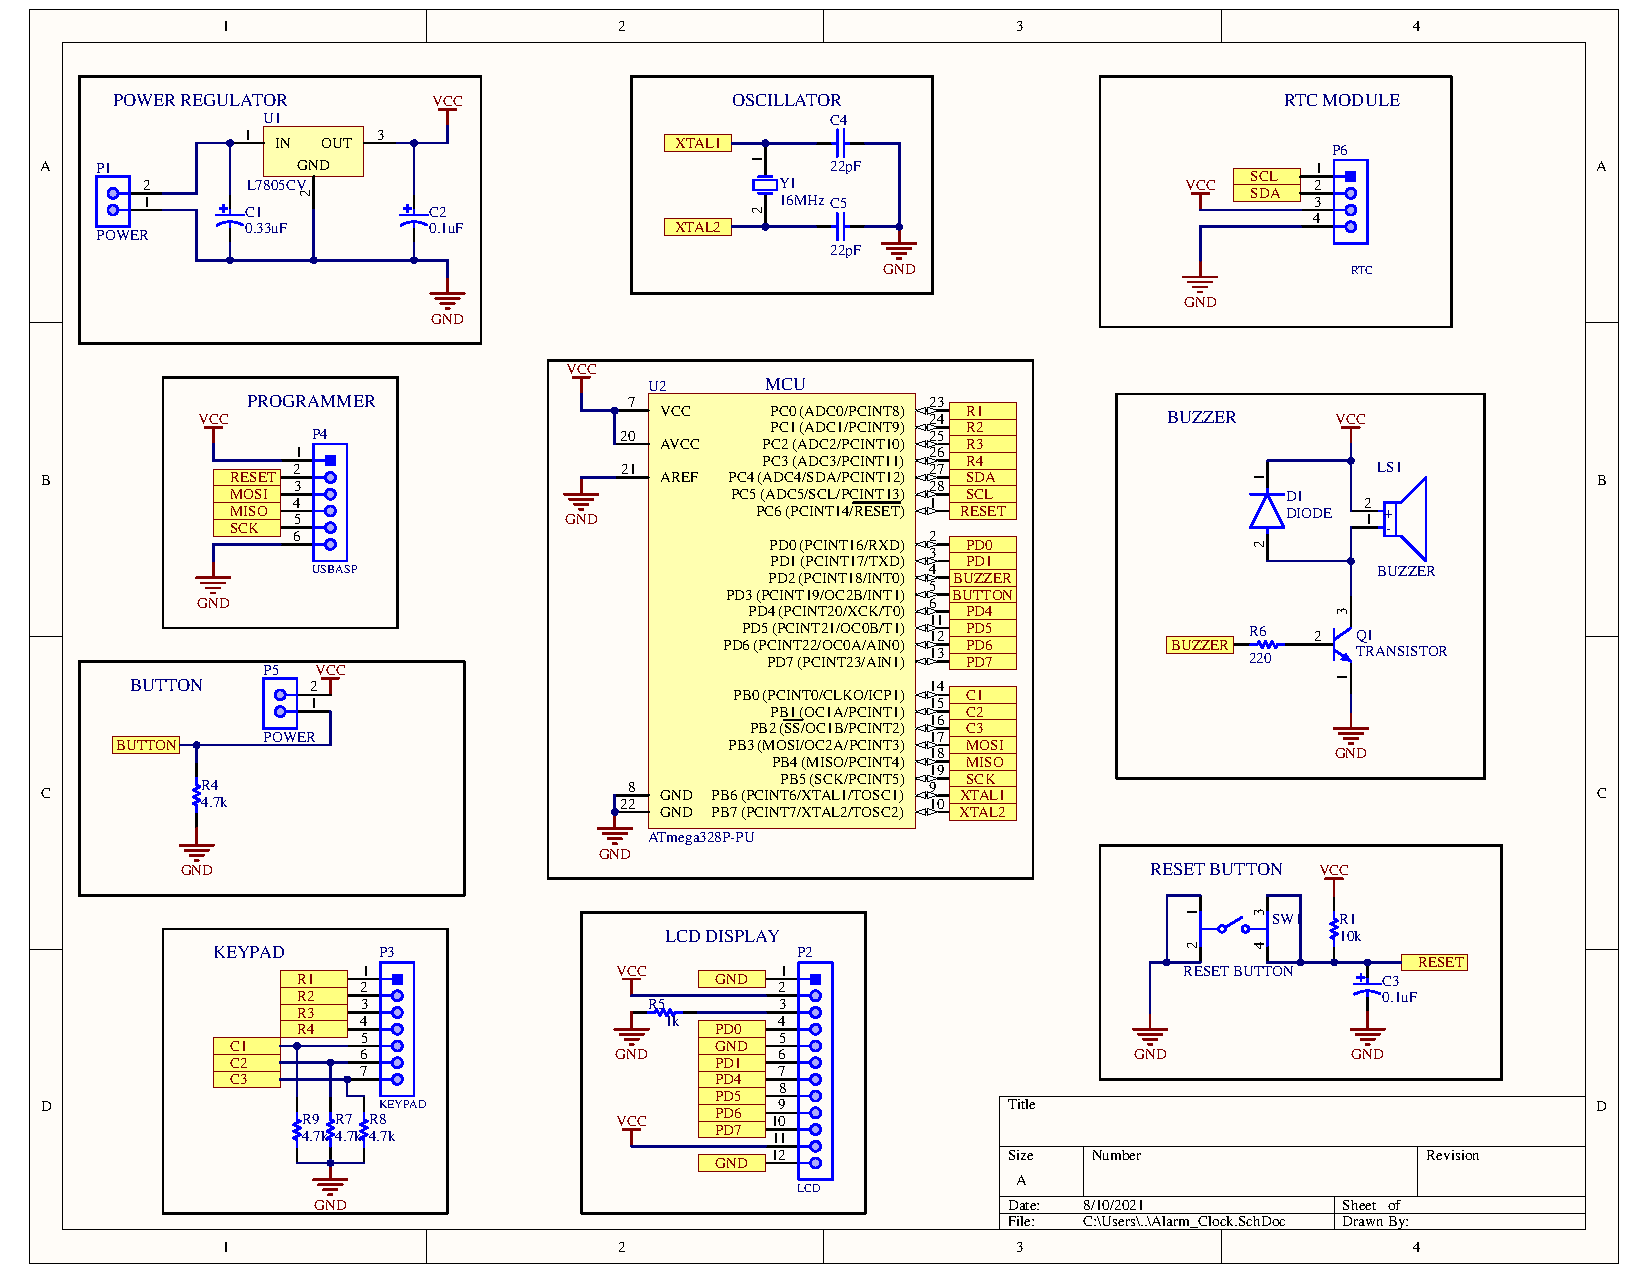
\includegraphics[]{Appendix/Alarm_Clock.pdf}
  \begin{figure}
  \noindent\makebox[\textwidth]{
  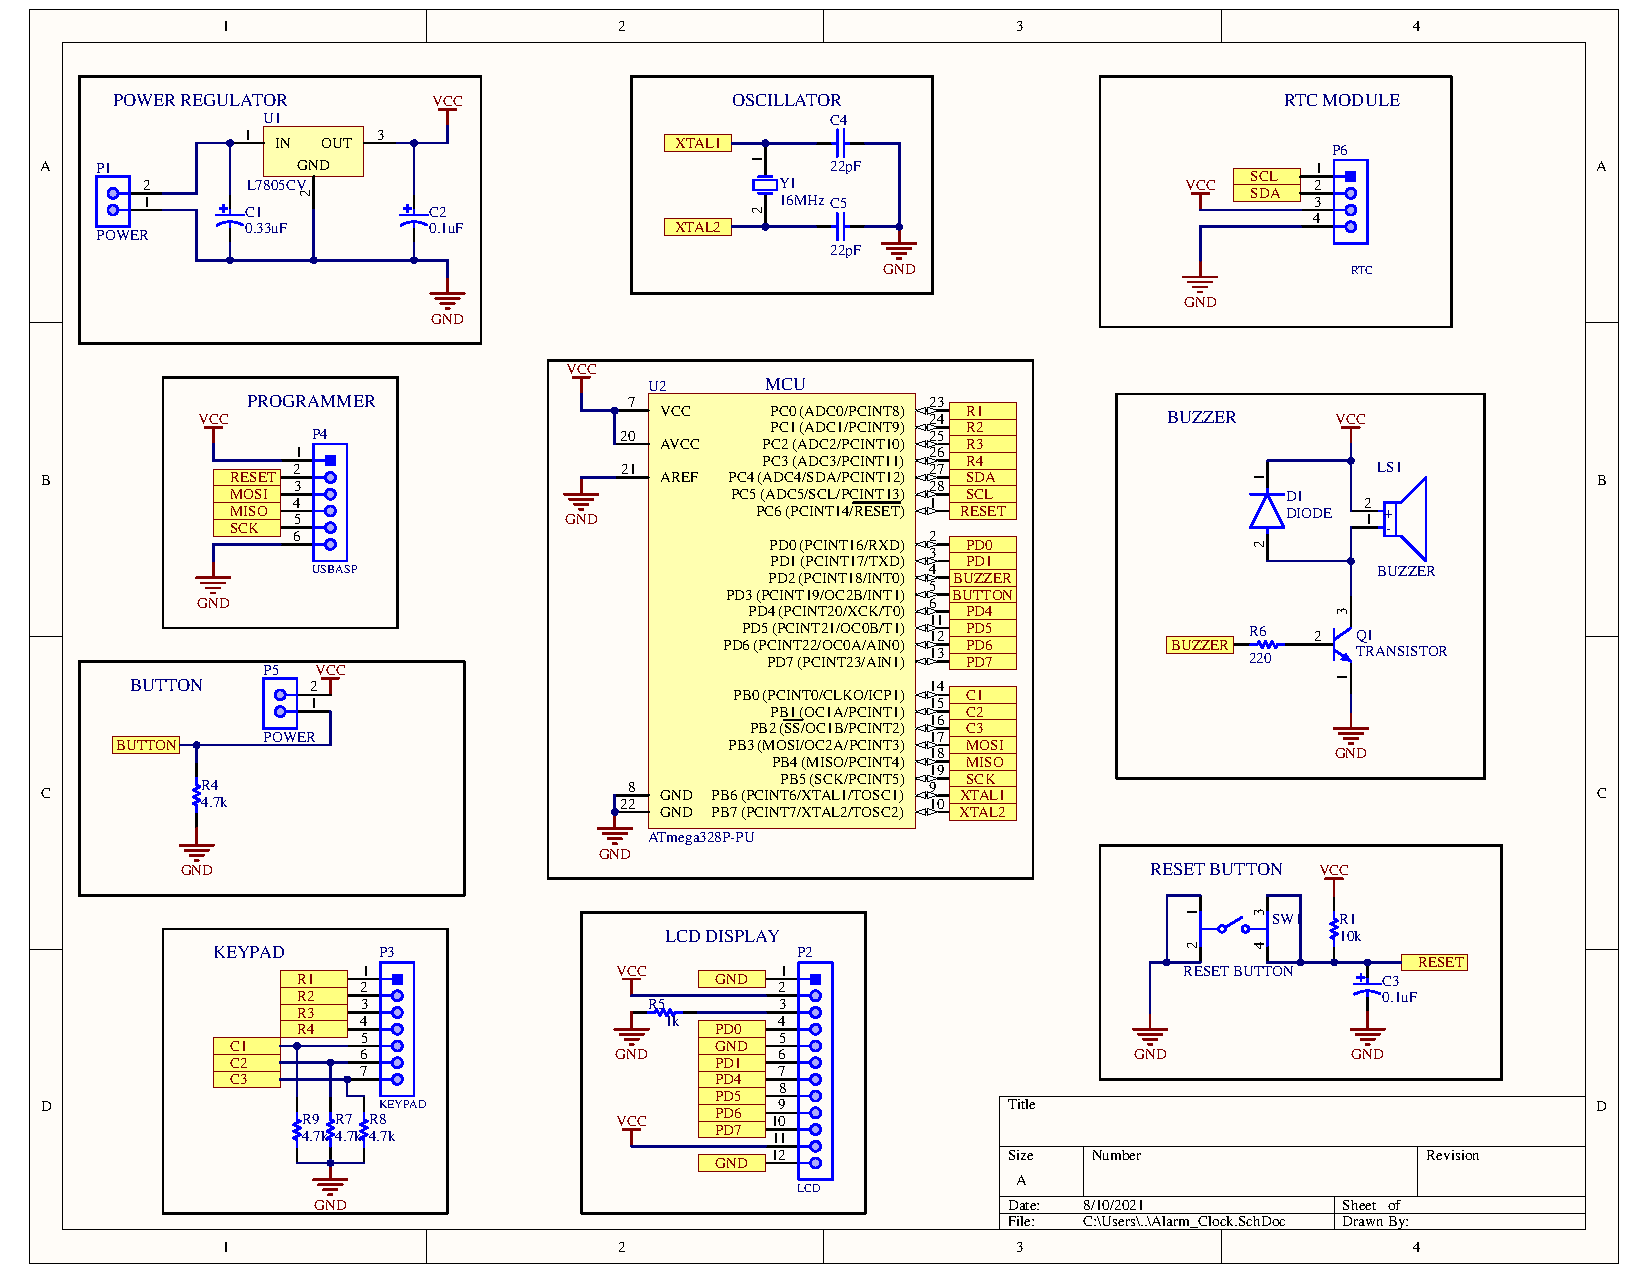
\includegraphics[width=1.3\textwidth,page=1]{Appendix/Alarm_Clock.pdf}}
  \caption{Schematics Design}
\end{figure}


\newpage

  \begin{figure}
  \noindent\makebox[\textwidth]{
  \includegraphics[width=1.4\textwidth,page=2]{Appendix/Alarm_Clock.pdf}}
  \caption{PCB Design}
\end{figure}

  \begin{figure}
  \noindent\makebox[\textwidth]{
  \includegraphics[width=1.7\textwidth,page=3]{Appendix/Alarm_Clock.pdf}}
  \caption{BOM}
\end{figure}

\newpage
\section{Proteus schematics}

  \begin{figure}[h]
  \noindent\makebox[\textwidth]{
  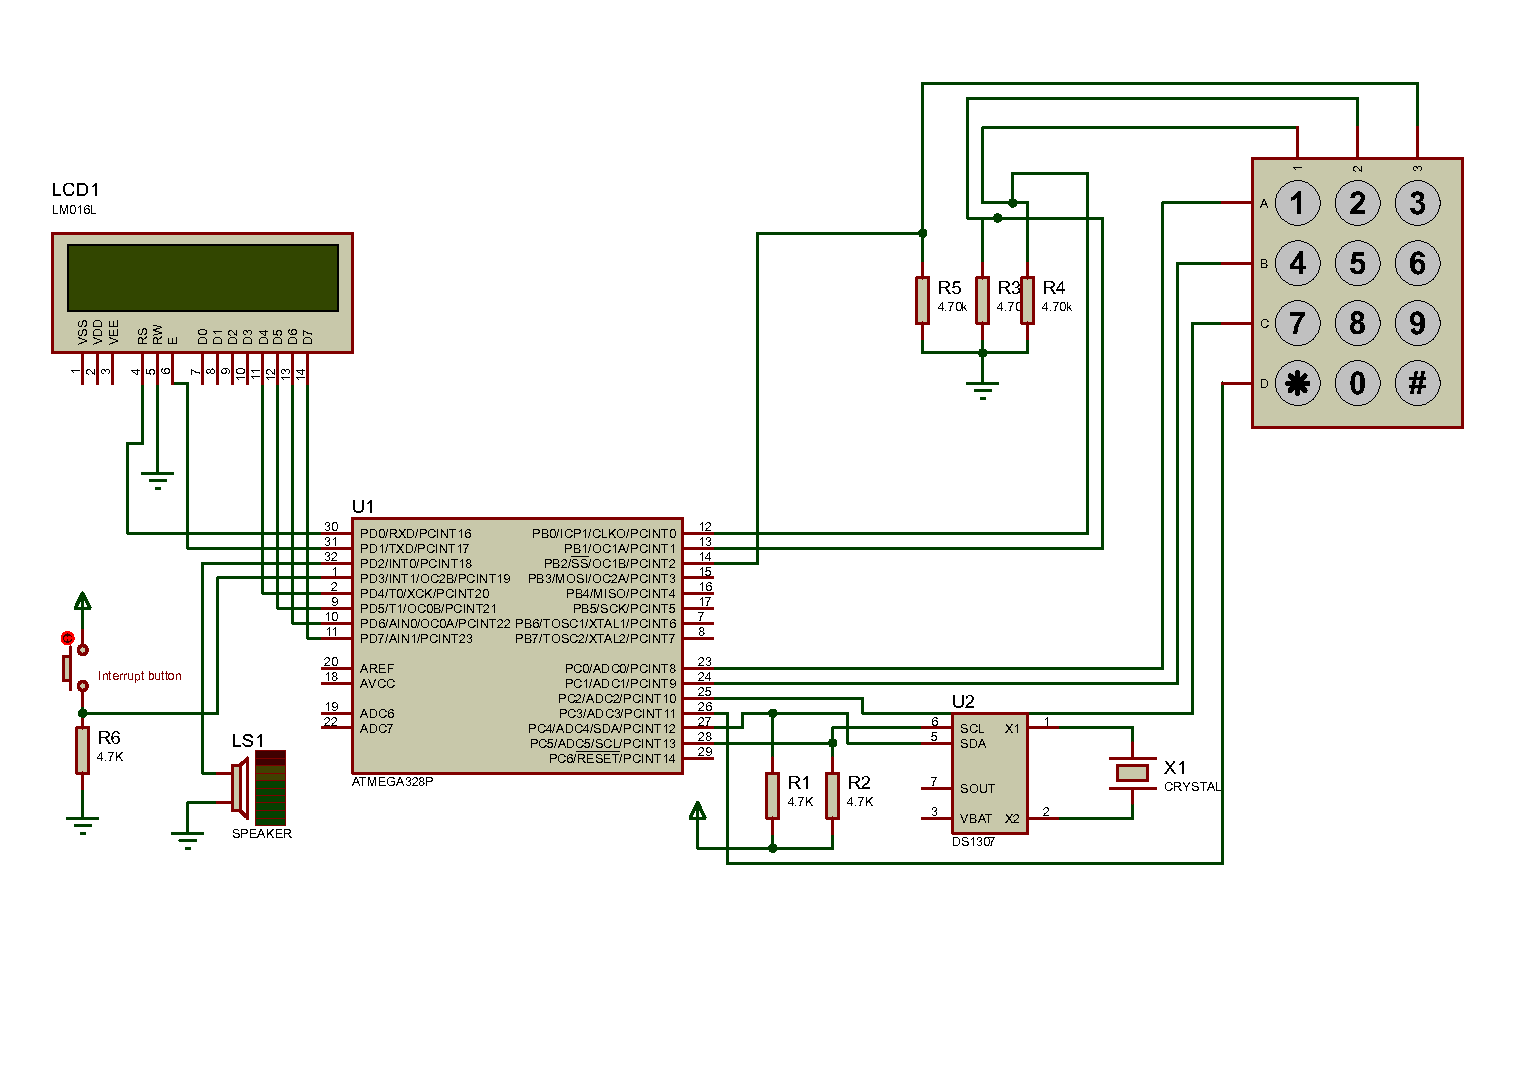
\includegraphics[width=1.4\textwidth,page=1]{Proteus.PDF}}
  \caption{Proteus Simulation}
\end{figure}
\newpage

\section{Enclosure}
\textcolor{red}{
Please use Adobe reader DC to view this. Also for better view, open in full screen by right clicking.}


\begin{minipage}{\linewidth}
\centering
\noindent\makebox[\textwidth]{
\includemedia[
label=my3d,
  width=1.2\linewidth,
  height=1.3\linewidth,activate=pageopen,
  3Dtoolbar,
  3Dmenu,
  3Daac=60,
  3Dcoo=1 1 1,
  3Droo=150,
  3Dlights=Headlamp,
]{}{utput.u3d}

}
\captionof{figure}{3D Enclosure View}
\end{minipage}

\newpage

\begin{minipage}{0.97\textwidth}
 \noindent\makebox[\textwidth]{
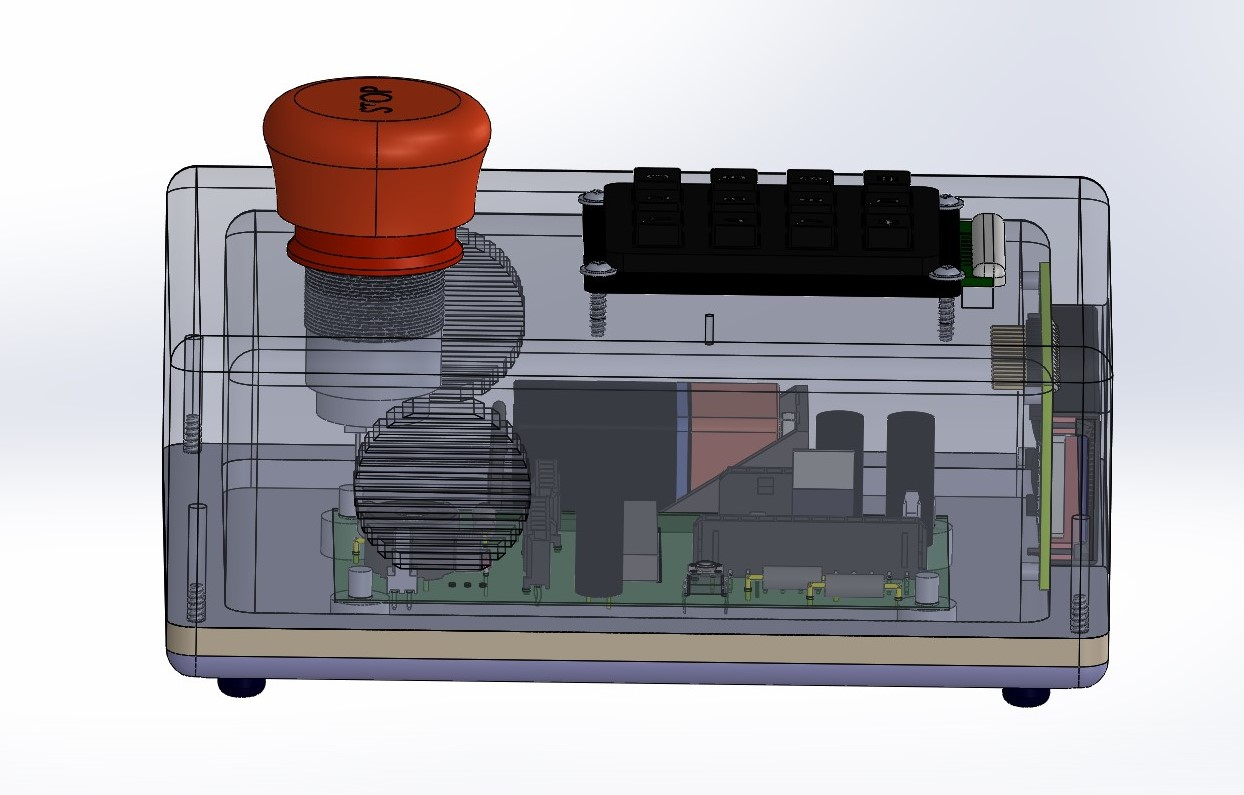
\includegraphics[width=0.5\textwidth]{Enclosure/trans1.jpg}
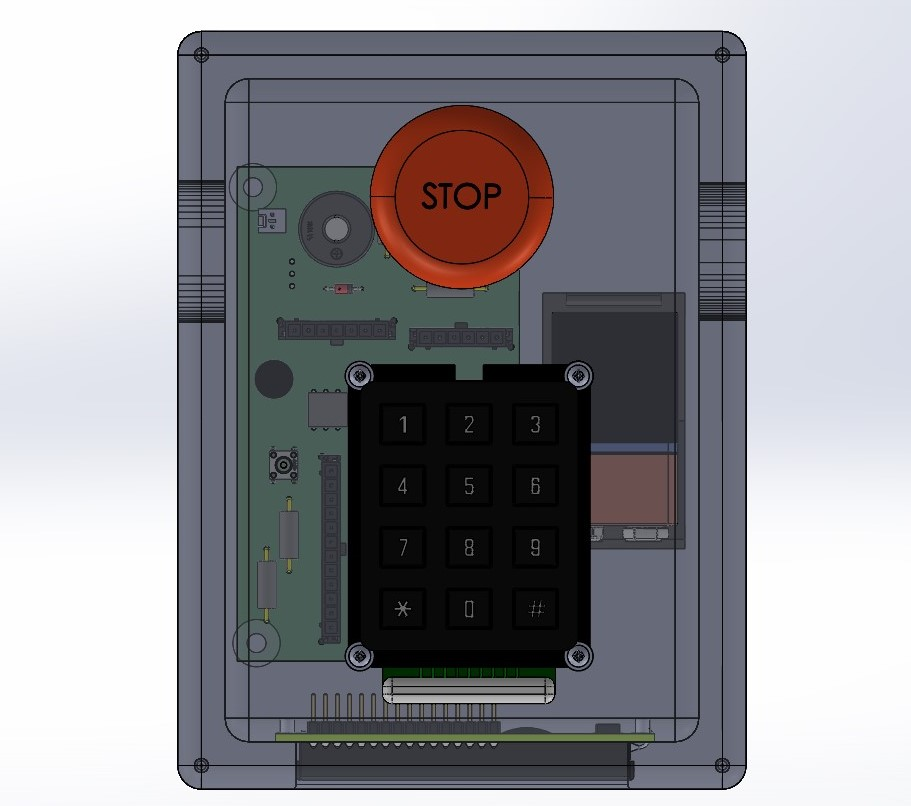
\includegraphics[width=0.5\textwidth]{Enclosure/trans2.jpg}}\hfill
\noindent\makebox[\textwidth]{
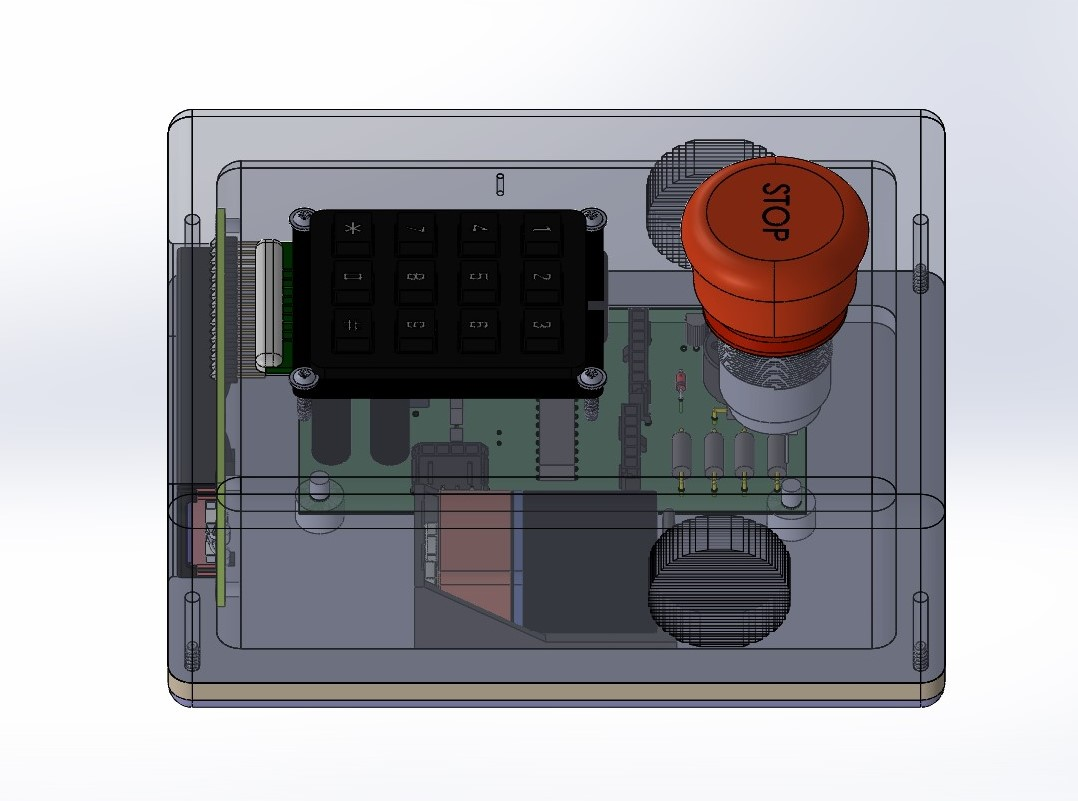
\includegraphics[width=0.5\textwidth]{Enclosure/trans3.jpg}
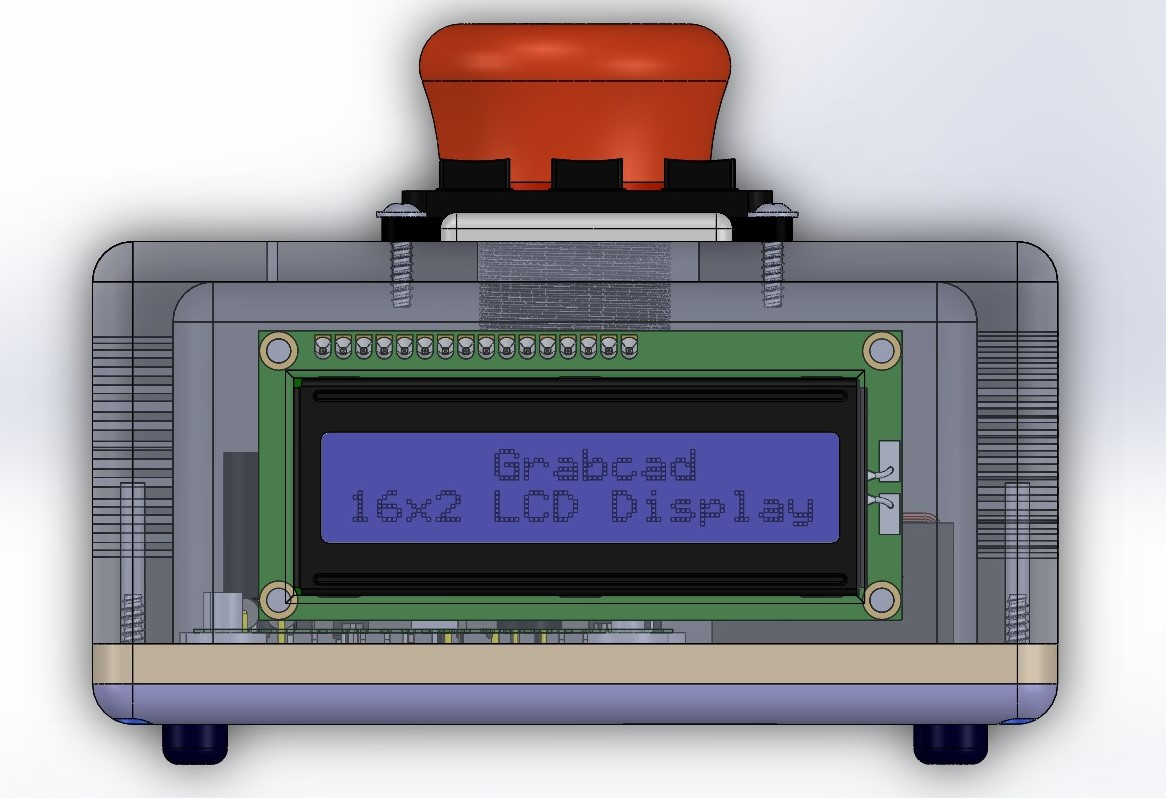
\includegraphics[width=0.5\textwidth]{Enclosure/trans4.jpg}}\hfill
\captionof{figure}{Transparent Enclosure views}
\end{minipage}

\newpage

\section{AVR Codes}
%\inputminted{cpp}{AVR/Alarm.cpp}

\lstinputlisting[language=C, caption={Main.ccp}]{AVR/Main.cpp}
\newpage

\lstinputlisting[language=C, caption={Alarm.h}]{AVR/Alarm.h}
\lstinputlisting[language=C, caption={Alarm.ccp}]{AVR/Alarm.cpp}
\lstinputlisting[language=c, caption={Buzzer.h}]{AVR/Buzzer.h}
\lstinputlisting[language=C, caption={Buzzer.ccp}]{AVR/Buzzer.cpp}
\lstinputlisting[language=C, caption={pitches.h}]{AVR/pitches.h}

\lstinputlisting[language=C, caption={melodies.h}]{AVR/melodies.h}
\newpage
\lstinputlisting[language=C, caption={Display.h}]{AVR/Display.h}
\lstinputlisting[language=C, caption={Display.cpp}]{AVR/Display.cpp}
\lstinputlisting[language=C, caption={Keypad.h}]{AVR/Keypad.h}
\lstinputlisting[language=C, caption={Keypad.cpp}]{AVR/Keypad.cpp}
\lstinputlisting[language=C, caption={ds1307.h}]{AVR/ds1307.h}
\lstinputlisting[language=C, caption={ds1307.cpp}]{AVR/ds1307.cpp}

\lstinputlisting[language=C, caption={i2cmaster.h}]{AVR/i2cmaster.h}
\lstinputlisting[language=C, caption={i2cmaster.cpp}]{AVR/i2cmaster.cpp}
